\documentclass[12pt]{article}
\usepackage{geometry}                % See geometry.pdf to learn the layout options. There are lots.
\geometry{a4paper}                   % ... or a4paper or a5paper or ... 
%\geometry{landscape}                % Activate for for rotated page geometry
%\usepackage[parfill]{parskip}    % Activate to begin paragraphs with an empty line rather than an indent
\usepackage{graphicx}
\usepackage{amssymb}
\usepackage{amsmath}
\usepackage{epstopdf}
\DeclareGraphicsRule{.tif}{png}{.png}{`convert #1 `dirname #1`/`basename #1 .tif`.png}

\usepackage{apacite}

\title{Text related to statistical analyses}
\author{Shravan Vasishth (vasishth@uni-potsdam.de)}
%\date{}                                           % Activate to display a given date or no date

\begin{document}
\maketitle
%\section{}
%\subsection{}

\section*{Statistical analysis methodology for CyTOF and RT-DC}

Statistical comparisons between groups can be carried out in the linear modeling setting by defining a so-called contrast coding \cite{venablesripley}. For example, when comparing means from two groups, the so-called sum-contrast can be used to  code one group as $-1$ and the other as $+1$.  This amounts to expressing the hypothesis that the mean of one group is identical to that of the other. When more than two groups (say, three groups labeled A, B, C) is present one approach for pairwise comparisons is to use the so-called sliding contrast or successive difference contrast to express that we want to compare group B with A, and group C with B. This contrast coding scheme can be applied to any number of groups. 

Given the CyTOF data for each leucocyte cell subset (T cells, Neutrophils, NK cells, Monocytes and B cells), 
we were interested in evaluating differences between the following groups: three GBCA, and three GBCA concentrations.  


The dependent variable is the Gd (Gd158 isotope) signal. The groups for RT-DC data are the cells (monocytes and neutrophils) and three GBCA at one concentration (1mM). The dependent variable here is the elastic Young's modulus variable.

The research question was whether GBCA binds the leucocyte cell subsets by assessment of CyTOF - Gd158 signal (CyTOF data), and whether the cellular attachment / uptake of GBCA induces cell deformability (RT-DC data).

Since the dependent measures in the CyTOF and RT-DC data came with an uncertainty interval (5th and 95th percentile), we took into account the uncertainty of each measurement by fitting a Bayesian hierarchical measurement error model \cite{Gelman14}. All the models were fit using the probabilistic programming language Stan, version 2.17.0 \cite{carpenter2017stan}, with the help of the software brms, version 2.1.9 \cite{brms}.  

The Bayesian framework is especially attractive in this particular data analysis situation for several reasons. First, as in the present case, when the data are relatively sparse, Bayesian models furnish robust estimates due to the presence of regularizing priors (explained below). Second, the end-product of a Bayesian analysis is the joint posterior distribution of the parameters. From this joint posterior, we can derive marginal distributions of each parameter and draw inferences from these. The focus here is not on significance testing but rather on quantifying uncertainty about each of the parameters. We will summarize the marginal distributions of the posteriors using the posterior means and 95\% credible intervals. These intervals demarcate the range over which we can be 95\% percent sure that the true value of the parameter lies, given the data and model.

Measurement error models take the uncertainty in the measurement of the dependent and/or independent variable into account \cite{clayton1992models,richardson1993bayesian}. As a simple example, if the dependent variable $y$ has standard error $s$, the true measurement $y_{true}$ can be treated as a missing variable: $y\sim Normal(y_{true}, s)$. The model is then fit with the missing variable $y_{true}$ as the dependent variable. 

The CyTOF model was defined as follows. Because we have repeated measures (from different cell types) for each contrast agent, we define a hierarchical model with a varying intercept for each cell type, and varying slopes by cell type for each predictor. 
The dependent variable is $\log(Mean)$, and the standard error on the measurement is SE (to-do: provide units). The predictors are (a) \texttt{logConc} is concentration on the log scale, (b)  a comparison of G(adovist) vs.\  M(agnevist), coded as \texttt{GvsM}, (c)  a comparison of M(agnevist) vs.\ D(otarem), coded GvsM, (d)  the interaction of   \texttt{logConc} and \texttt{GvsM}, and (e) the interaction of   \texttt{logConc} and \texttt{MvsD}. The adjustments by the $i$ cell type to the fixed effects coefficients are coded as $u_{0i},\dots, u_{5i}$; these induce variance components, described below.

\begin{equation}
\begin{split}
\log(Mean) \sim& Normal(\log(Mean)_{true}, SE)\\
\log(Mean)_{true} =& \beta_0 + u_{0i} + (\beta_1 + u_{1i})\hbox{logConc} + (\beta_2 + u_{2i}) GvsM +
(\beta_3 + u_{3i}) MvsD +\\
~& (\beta_4 + u_{4i}) GvsM\times  \hbox{logConc} + (\beta_5 + u_{5i})MvsD\times  \hbox{logConc} + \varepsilon\\
\end{split}
\end{equation}

Apart from the residual error $\varepsilon$, the variance components of the random effects are assumed to be generated from a multivariate normal with six dimensions:

\begin{equation}
\begin{split}
\varepsilon \sim & Normal(0,\sigma_e)\\
\left(
\begin{matrix}
u_0\\
u_1\\
u_2\\
u_3\\
u_4\\
u_5\\
\end{matrix}
\right)
\sim &
MVNormal_6\left( 
\left(
\begin{matrix}
0\\
0\\
0\\
0\\
0\\
0\\
\end{matrix}
\right)
,
\mathbf{\Sigma}_{6,6}
\right)\\
\end{split}
\end{equation}

The $6\times 6$ variance-covariance matrix contains the variances for each random effect term $u_{0},\dots, u_{5}$, along with the correlations between them. 

Because we fit a Bayesian hierarchical model, it is necessary to specify priors for each of the parameters. We describe these prior specifications next.

\begin{enumerate}
\item All the fixed-effects coefficients $\beta$ parameters have $Caucy(0,5)$ priors.  This prior allows a wide range of values around $0$. These are so-called mildly informative priors \cite{Gelman14}.
\item All the standard deviations have a $Normal(0,1)$ prior truncated at 0 (because standard deviations cannot be smaller than 0). This prior is also a mildly informative prior, and is reasonable given that the dependent measure is on the log scale.
\item The correlation matrix derived from the variance-covariance matrix $\mathbf{\Sigma}$ has special regularizing priors that are currently only available in Stan. These are called LKJ priors and they take a real number as a parameter. When this parameter is $2$, extreme values ($\pm 1$) for the correlations are  downweighted (hence the term regularizing prior), and most of the probability mass lies between $-1$ and $+1$. For details, see the Stan documentation \cite{stan-manual:2017}.
\end{enumerate}

These regularizing priors ensure that such hierarchical models will usually converge. This is a significant advantage over frequentist tools for fitting linear mixed models, where convergence or estimation problems often occur; for an example of estimation problems in the frequentist linear mixed model, see \cite{VasishthBeckmanetal}. 

\subsection*{Results: CyTOF}

The posterior distributions shown in Figure~\ref{fig:cytof}.  (to-do: Eric, can you interpret this?)

Each slope parameter shows a positive estimate. The figure shows that a unit increase of log concentration leads to an increase in the dependent variable of 0.8; all others parameters also show a positive coefficient. 

\begin{figure}[!htbp]
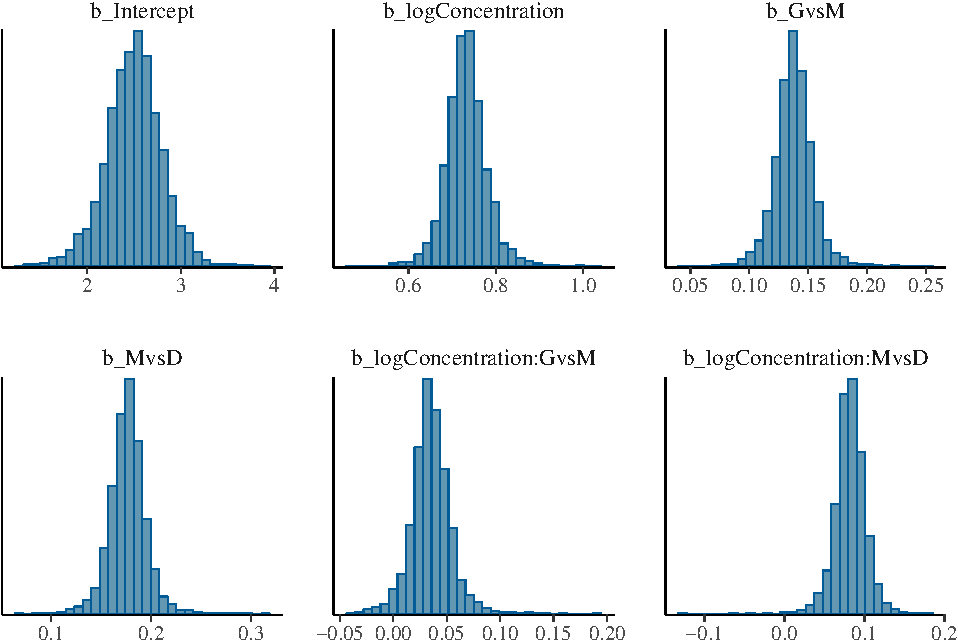
\includegraphics{cytof_brm_log-1}
\caption{Shown are the posterior distributions of the fixed effects parameters.}\label{fig:cytof}
\end{figure}

\bibliographystyle{apacite}
\bibliography{bibliography}

\end{document}  